\section{Advection} \label{sec:adv}
Advection is a fluid flow transporting something with it as it flows. This can be temperature, gas, solids or other fluids. In our case we will be looking at temperature.

\subsection{Thermal Diffusion}
As of this time, what you notice if you run the model is that the winds only get stronger and stronger (and the model is hence blowing up, which means that the numbers increase so dramatically 
that it is no longer realistic). This is because there is no link yet between the velocities of the atmosphere and the temperature. Currently, any air movement does not affect the temperature 
in the atmosphere of our model while it does in reality. So we need to change some calculations to account for that. Thermal diffusion helps with spreading out the temperatures and tempering 
the winds a bit.

The diffusion equation, as written in \autoref{eq:diffusion}, describes how the temperature spreads out over time\cite{diffusion}. The symbols in the equation represent:

\begin{itemize}
    \item $u$: A vector consisting out of 4 elements: $x, y, z, t$. $x, y, z$ are the local coordinates and $t$ is time.
    \item $\alpha$: The thermal diffusivity constant.
    \item $\nabla^2$: The Laplace operator, more information in \autoref{sec:laplace}.
    \item $\bar{u}$: The time derivative of $u$, or in symbols $\frac{\delta u}{\delta t}$.
\end{itemize}

\begin{equation}
    \bar{u} = \alpha \nabla^2 u
    \label{eq:diffusion}
\end{equation}

Now to get this into code we need the following algorithms \autoref{alg:laplacian} and \autoref{alg:diffusion}. \autoref{alg:laplacian} implements the laplacian operator, whereas 
\autoref{alg:diffusion} implements the diffusion calculations.  $\nabla^2$ in \autoref{alg:diffusion} represents the call to \autoref{alg:laplacian}.

\begin{algorithm}
    $T_a \leftarrow T_a + \delta t \alpha_a \nabla^2(T_a)$ \;
    $T_p \leftarrow T_p + \delta t \alpha_p \nabla^2(T_p)$ \;
    \caption{The main calculations for calculating the effects of diffusion}
    \label{alg:diffusion}
\end{algorithm}

\subsection{Adding in Advection}
With thermal diffusion in place, the temperature will spread out a bit, however air is not transported yet. This means that the winds we simulate are not actually moving any air. Advection is
going to change that. The advection equation is shown in \autoref{eq:advection}. The symbols are:

\begin{itemize}
    \item $\psi$: What is carried along (in our case temperature, \si{K}).
    \item $t$: The time (\si{s}).
    \item $u$: The fluid velocity vector (\si{ms^{-1}}).
    \item $\nabla$: The divergence operator (as explained in \autoref{sec:laplace}).
\end{itemize}

\begin{equation}
    \frac{\delta \psi}{\delta t} + \nabla \cdot (\psi u) = 0
    \label{eq:advection}
\end{equation}

With the divergence functon defined in \autoref{alg:divergence}, we now need to adjust \autoref{alg:diffusion} to incorporate this effect. The resulting algorithm can be found in 
\autoref{alg:advection}. Here $\nabla$ represents the function call to \autoref{alg:divergence}.

\begin{algorithm}
    $T_{add} \leftarrow T_a + \delta t \alpha_a \nabla^2(T_a) + \nabla(T_a)$ \;
    $T_a \leftarrow T_a + T_{add}[5:-5, :] \text{ //Only add } T_{add} \text{ to } T_a \text{ for indices in the interval } [-nlat + 5, nlat - 5]$. \;
    $T_p \leftarrow T_p + \delta t \alpha_p \nabla^2(T_p)$ \;
    \caption{The main calculations for calculating the effects of advection}
    \label{alg:advection}
\end{algorithm}

Now that we have the air moving, we also need to account for the moving of the density. This is because moving air to a certain place will change the air density at that place if the air at that 
place does not move away at the same rate. Say we are moving air to $x$ at $y \ ms^{-1}$. If air at $x$ moves at a rate $z \ ms^{-1}$ and $z \neq y$ then the air density at $x$ will change.
The equation we will need for that is the mass continuity equation as shown in \autoref{eq:mass continuity} \cite{masscontinue}.

\begin{equation}
    \frac{\delta \rho}{\delta t} + \nabla \cdot (\rho v) = 0
    \label{eq:mass continuity}
\end{equation}

Using this equation means that we will no longer assume that the atmosphere is incompressible. Therefore we need to change a few things in the code. First we need to change the $\rho$ in 
\autoref{alg:stream3}. Since $\rho$ is no longer constant we need to access the right value of $\rho$ by specifying the indices. So $\rho$ will change to $\rho[lat, lon]$. Furthermore we need
to calculate $\rho$ after the movement of air has taken place, so we need to change \autoref{alg:advection} as well to include the calculations for $\rho$. The new version can be found in 
\autoref{alg:advectionv2}. Again the $\nabla$ represents the call to \autoref{alg:divergence}.


\begin{algorithm}
    $T_{add} \leftarrow T_a + \delta t \alpha_a \nabla^2(T_a) + \nabla(T_a)$ \;
    $T_a \leftarrow T_a + T_{add}[5:-5, :] \text{ //Only add } T_{add} \text{ to } T_a \text{ for indices in the interval } [-nlat + 5, nlat - 5]$. \;
    $\rho \leftarrow \rho + \delta t \nabla \rho$ \;
    $T_p \leftarrow T_p + \delta t \alpha_p \nabla^2(T_p)$ \;
    \caption{The main calculations for calculating the effects of advection}
    \label{alg:advectionv2}
\end{algorithm}

Currently the advection does not work like it should. This is probably due to boundary issues, where we get too close to the poles and it starts freaking out there \cite{simon}. So to fix this 
we are going to define boundaries and assume that the advection only works within those boundaries. We only let it change by half of the values. The changes are incorporated in 
\autoref{alg:advectionfix}. The reason why we mention this seperately, in contrast to the other fixes that we have incorporated throughout the manual already, is the accompanying change with the 
boundary. 

\begin{algorithm}
        $T_{add} \leftarrow T_a + \delta t \alpha_a \nabla^2(T_a) + \nabla(T_a)$ \;
        $T_a \leftarrow T_a - 0.5T_{add}[adv\_bound:-adv\_boun, :] \text{ //Only subtract } T_{add} \text{ to } T_a \text{ for indices in the interval } [-nlat + adv\_boun, nlat - adv\_boun]$. \;
        $\rho[adv\_boun: -adv\_boun, :] \leftarrow \rho - 0.5(\delta t \nabla \rho) \text{ //Only change the density for indices in the interval } [-nlat + adv\_boun, nlat - adv\_boun]$ \;
        $T_p \leftarrow T_p + \delta t \alpha_p \nabla^2(T_p)$ \;
        \caption{The main calculations for calculating the effects of advection}
    \label{alg:advectionfix}
\end{algorithm}

\subsection{Layers, layers and layers}
With the atmospheric layers, and all matrices that have an extra dimension to account for it, we need to add the correct indices to the advection algorithm \autoref{alg:advectionfix}. Let us 
add it, with \autoref{alg:advection layer} as a result. Here the ':' means all indices of the 3 dimensional matrix. 

\begin{algorithm}
    $T_{add} \leftarrow T_a + \delta t \alpha_a \nabla^2(T_a) + \nabla(T_a)$ \;
    $T_a \leftarrow T_a - 0.5T_{add}[adv\_boun:-adv\_boun, :, :] \text{ //Only subtract } T_{add} \text{ to } T_a \text{ for indices in the interval } [-nlat + adv\_boun, nlat - adv\_boun]$. \;
    $\rho[adv\_boun: -adv\_boun, :, :] \leftarrow \rho - 0.5(\delta t \nabla \rho) \text{ //Only change the density for indices in the interval } [-nlat + adv\_boun, nlat - adv\_boun]$ \;
    $T_p \leftarrow T_p + \delta t \alpha_p \nabla^2(T_p)$ \;
    \caption{The main calculations for calculating the effects of advection}
    \label{alg:advection layer}
\end{algorithm}

First thing to mention is that vertical advection is still broken. Why? Because the gradient in the $z$ direction is broken. This is due to finite differencing on an exponential function. The way
we calculate the difference from one layer to the other is by differencing them (subtracting) which is always finite. Therefore we always get some inaccuracies. Usually that is fine, but with an 
exponential function the differences, you guessed it, become exponentially wrong. As such, the function would eventually be so far off that the model would blow up. So we need to fix it. To 
prevent a blow up, we have disabled the call to the gradient $z$ function in \autoref{alg:divergence}. This ensures that the horizontal bits still work, but the vertical stuff does not.
As always, we will try to fix this in the future. 

\subsection{Adiabatic Motion}
Up until now, we have been moving air and the density of the atmosphere. However we have not transported any temperature yet. What this means is that if we have a packet of air (see it as a box
filled with air, but the box is invisible) $P$ which is at the planet surface. There $P$ has temperature $T_1$. If we then move $P$ to a layer higher up in the atmosphere, $P$ will still have 
the same temperature, which is wrong because the density differs. Due to this difference, there is either more or less pressure applied to the box of air which means that $P$ will contract or 
expand. This obviously changes it's temperature as the air molecules are closer together/further away from each other. Therefore the energy spread is different which affects the temperature. 
For a visual representation, please consult \autoref{fig:thermal potential}.

\begin{figure}
    \centering
    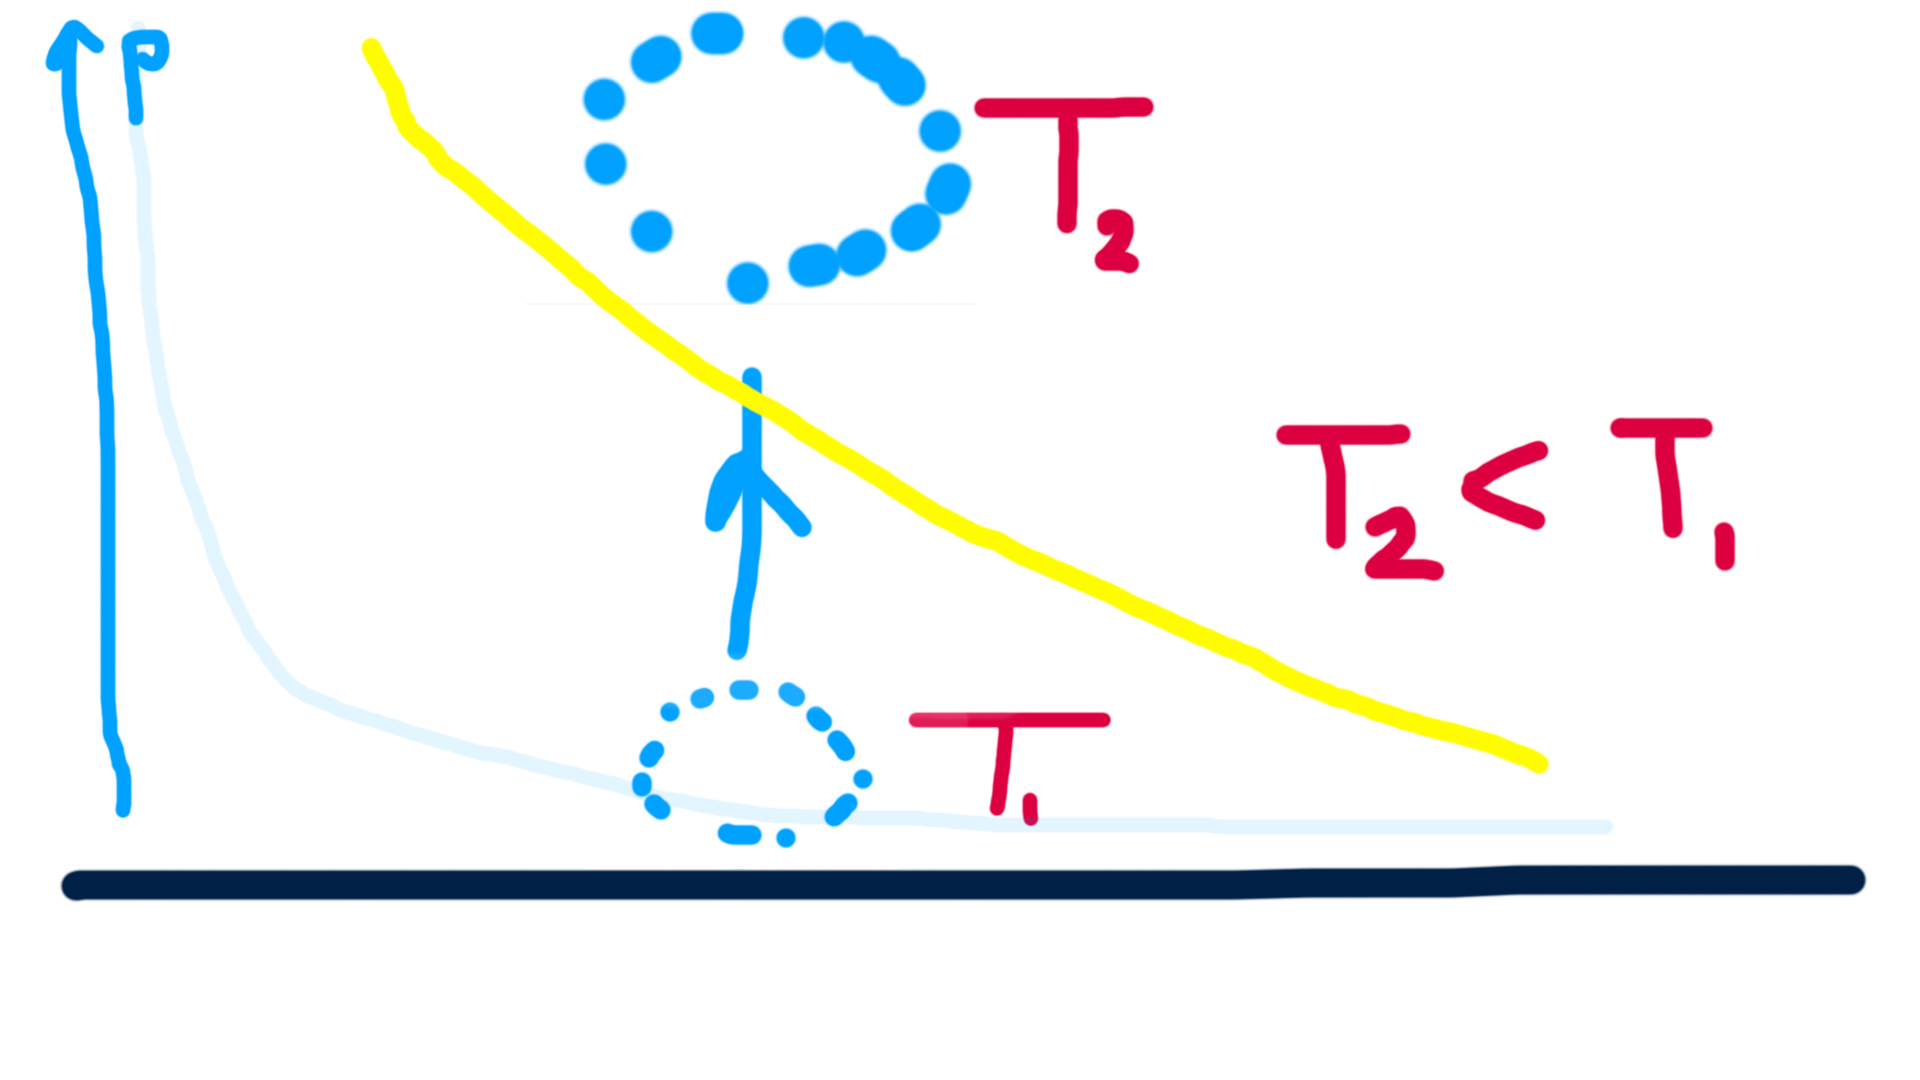
\includegraphics[width=0.9\textwidth]{figures/potential_temperature.jpg}
    \caption{Visual representation of why we need Thermal Potential \cite{simon}.}
    \label{fig:thermal potential}
\end{figure}

As seen in \autoref{fig:thermal potential}, the packet of air (next to $T_1$) moves up into a higher layer of the atmosphere and ends up at the top (next to $T_2$). The packet has grown bigger, 
as the density in that atmospheric layer is lower and hence the air expands. Because the same energy is in that packet, but it has expanded, the temperature of that packet drops which gives us 
$T_2 < T_1$. The light blue graph in the background shows how the density behaves the higher you go, meaning at the far right (when we are at the highest point) the density is quite low and at 
the far left (when we are at the planet surface) the density is quite high. The yellow graph shows the temperature of the air at that height, which behaves similarly to the density graph.

Thermal potential or potential temperature, is the temperature that the packet of air would be if it is at the planet surface. So take the packet at $T_2$ in \autoref{fig:thermal potential}. If we move that down to the 
surface, then it would be temperature $T$ which is then equal to the thermal potential. The equation corresponding to thermal potential is shown in \autoref{eq:thermal potential} 
\cite{thermalPotential}. The symbols in \autoref{eq:thermal potential} mean:

\begin{itemize}
    \item $T$: The temperature of the packet of air (\si{K}).
    \item $p_0$: Reference pressure, usually the pressure at the planet surface (\si{Pa}).
    \item $p$: Pressure of the packet of air (\si{Pa}).
    \item $R$: Gas constant as defined in \autoref{sec:gas constant} (\si{JK^{-1}mol^{-1}}).
    \item $C_a$: Specific heat capacity of air at a constant pressure (\si{Jkg^{-1}K^{-1}}).
\end{itemize}

\begin{subequations}
    \begin{equation}
        \theta = T(\frac{p_0}{p})^{\frac{R}{C_a}}
        \label{eq:thermal potential}
    \end{equation}
    \begin{equation}
        T = \theta(\frac{p}{p_0})^{\frac{R}{C_a}}
        \label{eq:potential temp}
    \end{equation}
\end{subequations}

If we now re-arrange \autoref{eq:thermal potential} so that we have $T$ on one side and the rest on the other side, we get \autoref{eq:potential temp}. With this we can convert temperature into 
potential temperature and vice versa. The whole process of moving temperature around is called adiabatic motion. Now it is time to get this into code. For this to work we need to translate both 
\autoref{eq:thermal potential} and \autoref{eq:potential temp} into code and create an overarching function that calls the previously mentioned equations. Let us start with 
\autoref{eq:thermal potential} which is described in \autoref{alg:temp to pot}. Note that $\frac{R}{C_a}$ does not change as they are constants, therefore we can precompute them which saves quite 
a bit of time (namely $O(n^3)$ divisions, where $n$ is the length of each dimension of $T_a$). Also note that we can inverse the process by inserting a minus in the exponent and swapping $T_a$ 
and $\theta$, which can easily be done in the call to \autoref{alg:temp to pot}. To avoid confusion we rename $p_0$ to $p_r$ as we talk about a reference pressure, instead of the already defined
pressure from a previous calculation round.

\begin{algorithm}
    \SetKwInOut{Input}{Input}
    \SetKwInOut{Output}{Output}
    \Input{temperature of the atmosphere $T_a$, air pressure $p$, boolean $back$}
    \Output{potential temperature $\theta$}
    \uIf{$back$}{
        $\kappa \leftarrow -\frac{R}{C_a}$ \;
    }\uElse{
        $\kappa \leftarrow \frac{R}{C_a}$ \;
    }
    \For{$i \leftarrow 0$ \KwTo $T_a.length$}{
        \For{$j \leftarrow 0$ \KwTo $T_a[i].length$}{
            $p_r \leftarrow p[i, j 0]$ \;
            \For{$k \leftarrow 0$ \KwTo $T_a[i, j].length$}{
                $\theta[i, j, k] \leftarrow T_a[i, j, k] (\frac{p[i, j, k]}{p_r})^{\kappa}$
            }
        }
    }
    \Return{$\theta$}
    \caption{Converting temperature into potential temperature}
    \label{alg:temp to pot}
\end{algorithm}

With that done we now only need to create the overarching function that will call \autoref{alg:temp to pot}. This function will be based on \autoref{alg:divergence} as it is quite similar for 
what we need to do, however we need to replace a call so we do need to make it a seperate function. Let us do that in \autoref{alg:thermal pot}. Here \texttt{TToTheta} represents the call to 
\autoref{alg:temp to pot}.

\begin{algorithm}[!hbt]
    \SetKwInOut{Input}{Input}
    \SetKwInOut{Output}{Output}
    \Input{temperature of the atmosphere $T_a$, pressure $p$}
    \Output{temperature of the atmosphere after advection $output$}
    $\theta \leftarrow $ \texttt{TToTheta}($T_a, p,$ \texttt{FALSE}) \;
    \For{$i \leftarrow 0$ \KwTo $a.length$}{
        \For{$j \leftarrow 0$ \KwTo $a[i].length$}{
            \For{$k \leftarrow 0$ \KwTo $a[i, j].length$}{
                $output[i, j, k] \leftarrow \Delta_x(\theta u, i, j, k) + \Delta_y(\theta v, i, j, k) + \Delta_z(\theta w, i, j, k)$ \;
            }
        }
    }
    $output \leftarrow $ \texttt{TToTheta}($output, p,$ \texttt{TRUE}) \;
    \Return{$output$} \;
    \caption{Calculate the result of the thermal advection}
    \label{alg:thermal pot}
\end{algorithm}

Now we only need to do one more thing, replace the algorithm that calculates $T_a$ as a result of advection. Let us do that in \autoref{alg:advection pot}, where \texttt{ThermalAdv} is the call 
to \autoref{alg:thermal pot}.

\begin{algorithm}
    $T_{add} \leftarrow T_a + $ \texttt{ThermalAdv}$(T_a, p)$\;
    $T_a \leftarrow T_a - 0.5T_{add}[adv\_boun:-adv\_boun, :, :] \text{ //Only subtract } T_{add} \text{ to } T_a \text{ for indices in the interval } [-nlat + adv\_boun, nlat - adv\_boun]$. \;
    $\rho[adv\_boun: -adv\_boun, :, :] \leftarrow \rho - 0.5(\delta t \nabla \rho) \text{ //Only change the density for indices in the interval } [-nlat + adv\_boun, nlat - adv\_boun]$ \;
    $T_p \leftarrow T_p + \delta t \alpha_p \nabla^2(T_p)$ \;
    \caption{The main calculations for calculating the effects of advection}
    \label{alg:advection pot}
\end{algorithm}